\section{Parâmetros físicos do manipulador robótico}
\label{ApendiceA}
A seguir, são listadas as características físicas dos elos que compõem o manipulador robótico, incluindo dimensões e massas. Todas as unidades estão apresentadas no Sistema Internacional (SI).

\begin{figure}[ht]
    \centering
    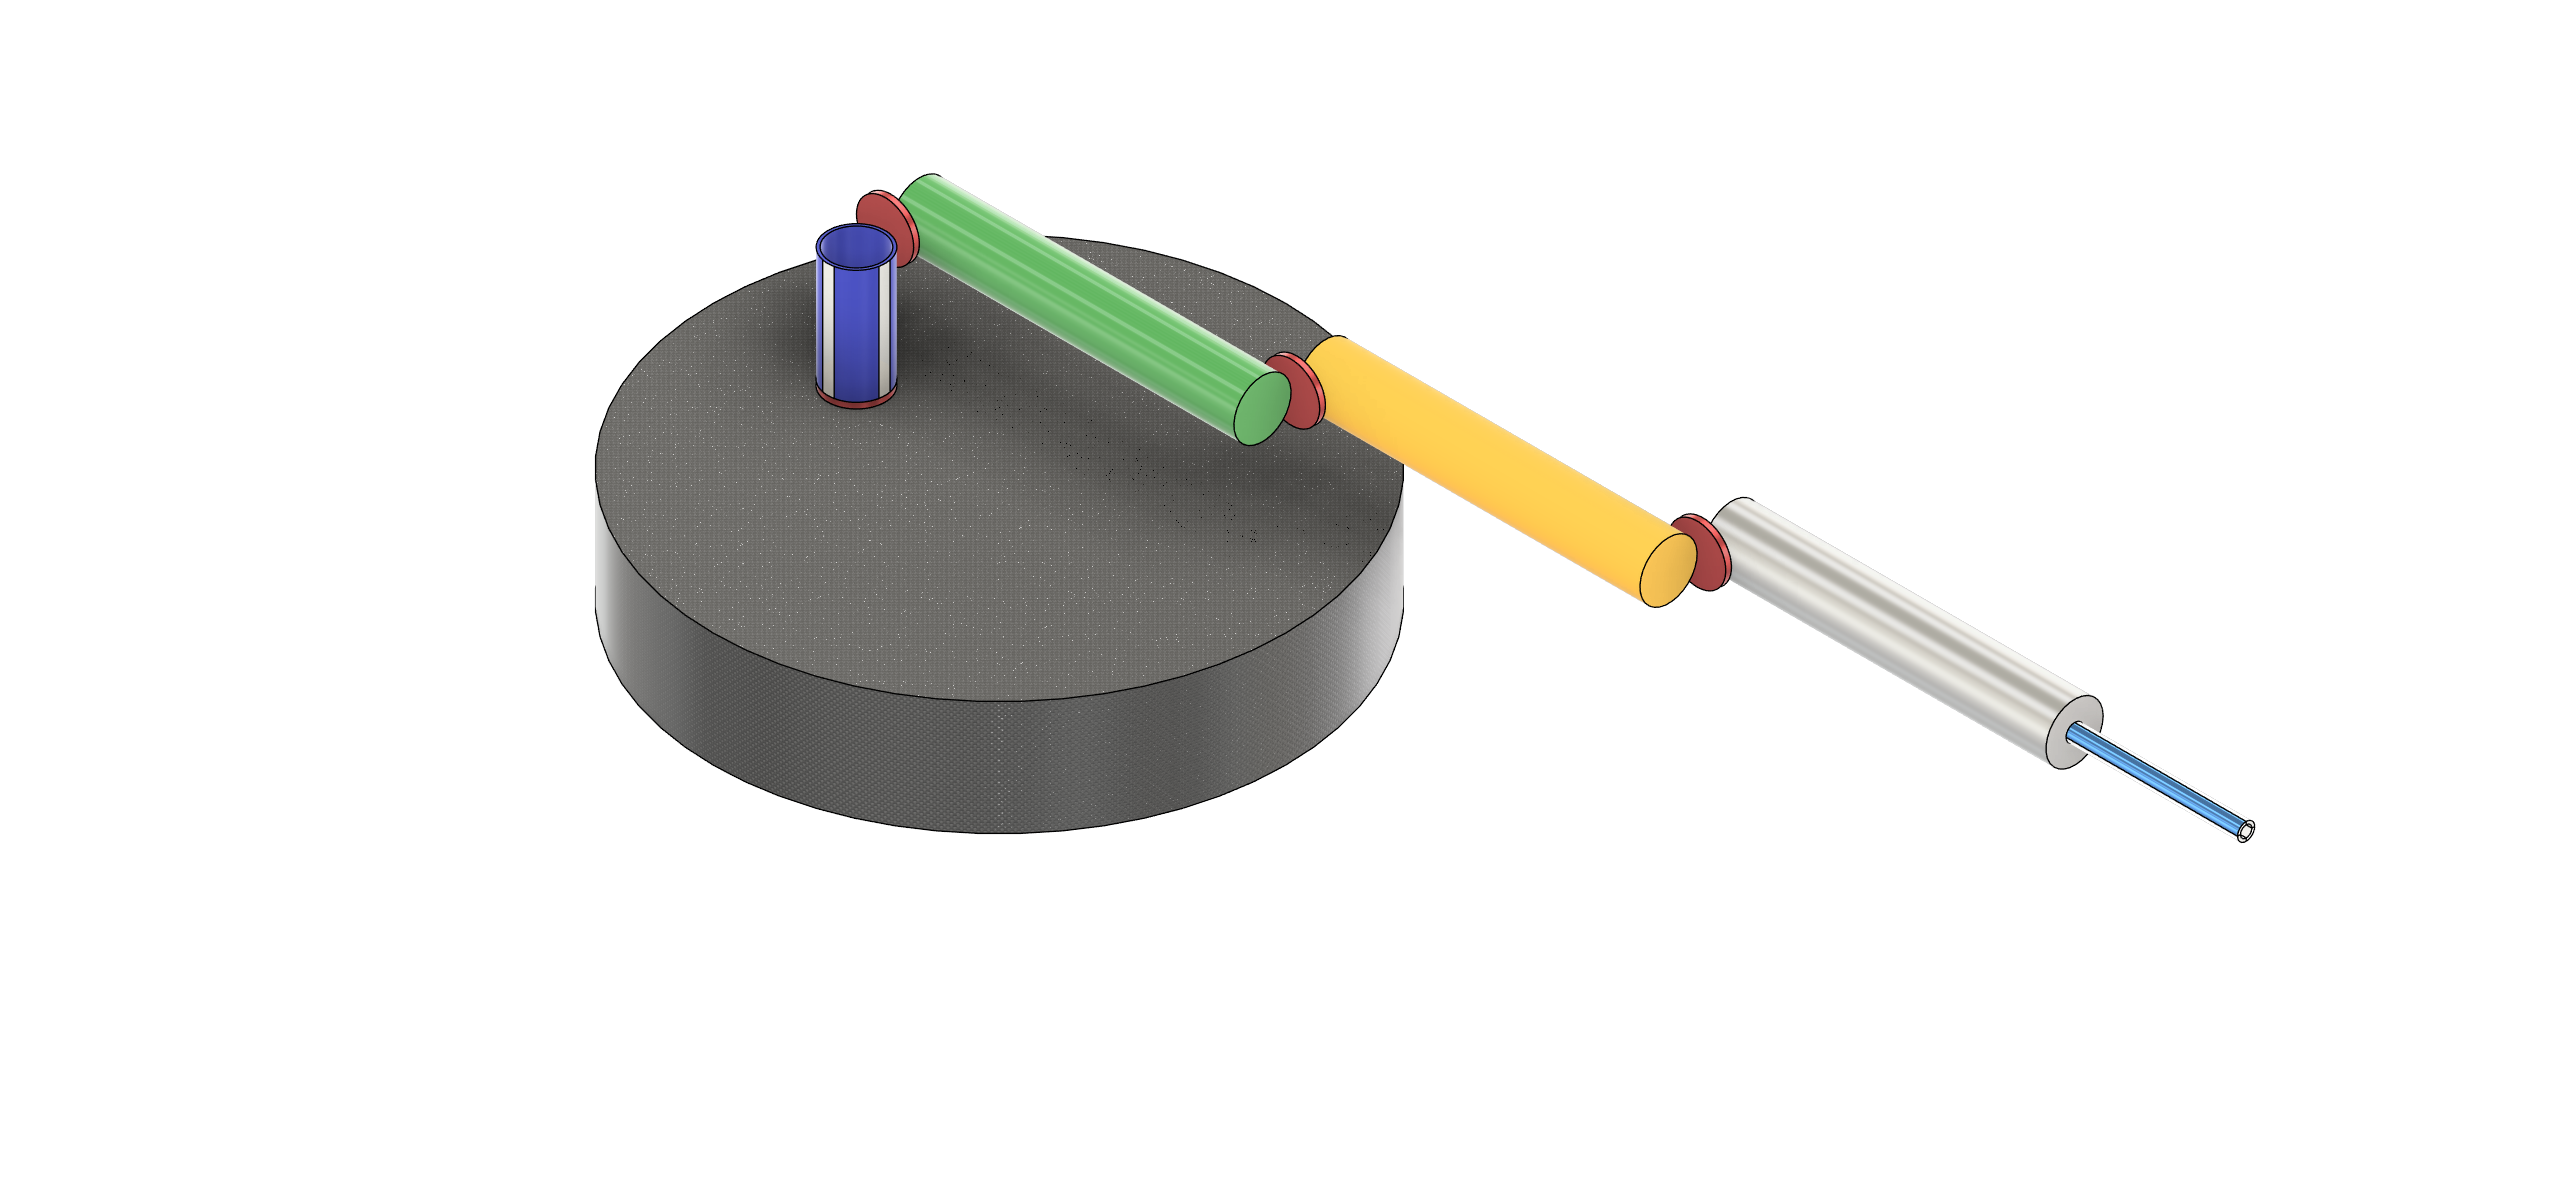
\includegraphics[width=0.9\textwidth]{2 Formulacao do problema/Imagens/Manipulador robotico 3D.png}
    \caption{Imagem digital do manipulador robótico desenvolvido pelo autor.}
    \label{fig:manipuladorRobotico_3D}
\end{figure}

\begin{table}[H]
\centering
\caption{Características físicas dos elos do manipulador robótico.}
\label{tab:elos_MR}
\begin{tabular}{lcc}
\toprule
Componente & Comprimento [m] & Raio externo [m] \\
\midrule
Elo 1      & 0,1000 & 0,0250 \\
Elo 2      & 0,3000 & 0,0250 \\
Elo 3      & 0,3000 & 0,0250 \\
Elo 4      & 0,3000 & 0,0250 \\
Ferramenta & 0,1500 & 0,0250 \\
\bottomrule
\end{tabular}
\end{table}

\section{Considerações sobre as Matrizes de Inércia}
As matrizes de inércia dos componentes do manipulador robótico foram obtidas a partir do software de modelagem tridimensional \emph{Autodesk Fusion 360} e estão expressas em unidades do Sistema Internacional (kg·m²).
Por se tratar de um manipulador leve, construído predominantemente em alumínio (densidade de $2.700\,\text{kg/m}^3$) e com dimensões reduzidas (elos ocos com espessura de parede de $0,0025\,\text{m}$), os valores numéricos resultantes podem parecer próximos de zero quando expressos em notação científica.

Tais valores não representam ausência de inércia, mas sim refletem a baixa massa e o pequeno raio de giro dos corpos em torno de seus eixos principais. Ainda assim, são relevantes para análises dinâmicas, especialmente em microgravidade ou em manobras de controle de alta precisão. Por isso, todas as matrizes de inércia foram integralmente mantidas nos modelos computacionais e nas simulações subsequentes.

\section{Parâmetros do Manipulador Robótico}
Nesta seção são apresentados os principais parâmetros físicos e geométricos do manipulador robótico desenvolvido.  
Os dados foram agrupados em quatro categorias:
\emph{centros de massa} (Tabela \ref{tab:com_manipulador}),
\emph{dimensões físicas} (Tabela \ref{tab:parametros_fisicos1}),
\emph{matrizes de inércia} (Tabelas \ref{tab:mi_diag} e \ref{tab:mi_foraDiag}),
e
\emph{limites operacionais das juntas} (Tabela \ref{tab:limites_manipulador}).

\begin{table}[ht]
\centering
\caption{Coordenadas dos centros de massa (SI).}
\label{tab:com_manipulador}
\begin{tabular}{lrrr}
\toprule
\textbf{Elemento} & \textbf{X [m]} & \textbf{Y [m]} & \textbf{Z [m]} \\
\midrule
Base Geral         & $9{,}202\times 10^{-12}$ & 0,0000 & 0,0500 \\
Junta 1            & $-5{,}259\times 10^{-12}$ & -0,1250 & 0,1025 \\
Junta 2            & -0,0275 & -0,1250 & 0,2050 \\
Junta 3            & -0,0825 & 0,1750  & 0,2050 \\
Junta 4            & -0,1375 & 0,4750  & 0,2050 \\
Elo 1              & $1{,}768\times 10^{-11}$ & -0,1250 & 0,1503 \\
Elo 2              & -0,0550 & 0,0301  & 0,2050 \\
Elo 3              & -0,1100 & 0,3301  & 0,2050 \\
Elo 4              & -0,1650 & 0,6301  & 0,2050 \\
Ferramenta         & -0,1650 & 0,8490  & 0,2050 \\
Manipulador Global & -0,0240 & 0,0703  & 0,0864 \\
\bottomrule
\end{tabular}
\end{table}

\begin{table}[H]
\centering
\caption{Dimensões físicas e massas dos componentes (SI).}
\label{tab:parametros_fisicos1}
\begin{tabular}{lrrrr}
\toprule
Componente & Altura [m] & Raio [m] & Diâmetro [m] & Massa [kg] \\
\midrule
Base Geral   & 0,1000 & 0,0250 & 0,0500 & 3,653 \\
Junta 1      & 0,0050 & 0,0250 & 0,0500 & 0,0265 \\
Junta 2      & 0,0050 & 0,0250 & 0,0500 & 0,0265 \\
Junta 3      & 0,0050 & 0,0250 & 0,0500 & 0,0265 \\
Junta 4      & 0,0050 & 0,0250 & 0,0500 & 0,0265 \\
Elo 1        & 0,1000 & 0,0250 & 0,0500 & 0,1115 \\
Elo 2        & 0,3000 & 0,0250 & 0,0500 & 0,3129 \\
Elo 3        & 0,3000 & 0,0250 & 0,0500 & 0,3129 \\
Elo 4        & 0,3000 & 0,0250 & 0,0500 & 0,3129 \\
Ferramenta   & 0,1500 & 0,0075 & 0,0150 & 0,0403 \\
\midrule
Massa Total &&&& 4,8495 \\
\bottomrule
\end{tabular}
\end{table}

\begin{table}[H]
\centering
\caption{Elementos diagonais das matrizes de inércia (kg·m$^{2}$).}
\label{tab:mi_diag}
\begin{tabular}{lrrr}
\toprule
Componente & $I_{xx}$ & $I_{yy}$ & $I_{zz}$ \\
\midrule
Base Geral   & $7,948\times 10^{-2}$ & $7,948\times 10^{-2}$ & $1,449\times 10^{-1}$ \\
Junta 1      & $4,197\times 10^{-6}$ & $4,197\times 10^{-6}$ & $8,283\times 10^{-6}$ \\
Junta 2      & $8,283\times 10^{-6}$ & $4,197\times 10^{-6}$ & $4,197\times 10^{-6}$ \\
Junta 3      & $8,283\times 10^{-6}$ & $4,197\times 10^{-6}$ & $4,197\times 10^{-6}$ \\
Junta 4      & $8,283\times 10^{-6}$ & $4,197\times 10^{-6}$ & $4,197\times 10^{-6}$ \\
Elo 1        & $1,368\times 10^{-4}$ & $1,368\times 10^{-4}$ & $5,969\times 10^{-5}$ \\
Elo 2        & $2,582\times 10^{-3}$ & $1,736\times 10^{-4}$ & $2,582\times 10^{-3}$ \\
Elo 3        & $2,582\times 10^{-3}$ & $1,736\times 10^{-4}$ & $2,582\times 10^{-3}$ \\
Elo 4        & $2,582\times 10^{-3}$ & $1,736\times 10^{-4}$ & $2,582\times 10^{-3}$ \\
Ferramenta   & $7,820\times 10^{-5}$ & $1,622\times 10^{-6}$ & $7,820\times 10^{-5}$ \\
Global       & $2,807\times 10^{-1}$ & $1,126\times 10^{-1}$ & $3,381\times 10^{-1}$ \\
\bottomrule
\end{tabular}
\end{table}

\begin{table}[H]
\centering
\caption{Elementos fora da diagonal das matrizes de inércia (kg·m$^{2}$).}
\label{tab:mi_foraDiag}
\begin{tabular}{lrrr}
\toprule
Componente & $I_{xy}$ & $I_{xz}$ & $I_{yz}$ \\
\midrule
Base Geral   & $6,601\times 10^{-16}$ & $1,639\times 10^{-12}$ & $-1,297\times 10^{-16}$ \\
Junta 1      & $-2,246\times 10^{-16}$ & 0 & 0 \\
Junta 2      & $-1,128\times 10^{-17}$ & 0 & 0 \\
Junta 3      & $-1,417\times 10^{-16}$ & $1,830\times 10^{-16}$ & $-1,249\times 10^{-15}$ \\
Junta 4      & $3,084\times 10^{-16}$ & $-1,323\times 10^{-17}$ & $-4,345\times 10^{-16}$ \\
Elo 1        & 0 & $-1,172\times 10^{-14}$ & $1,315\times 10^{-17}$ \\
Elo 2        & $2,138\times 10^{-15}$ & $-1,076\times 10^{-15}$ & $2,389\times 10^{-14}$ \\
Elo 3        & $9,663\times 10^{-17}$ & $-6,585\times 10^{-15}$ & $4,412\times 10^{-14}$ \\
Elo 4        & $6,325\times 10^{-14}$ & $4,290\times 10^{-15}$ & $-1,165\times 10^{-15}$ \\
Ferramenta   & $5,427\times 10^{-15}$ & $4,384\times 10^{-16}$ & $-5,684\times 10^{-16}$ \\
Global       & $4,390\times 10^{-2}$  & $1,381\times 10^{-2}$  & $-4,151\times 10^{-2}$ \\
\bottomrule
\end{tabular}
\end{table}

\begin{table}[H]
\centering
\caption{Limites de rotação e velocidade angular das juntas.}
\label{tab:limites_manipulador}
\begin{tabular}{ccc}
\toprule
Junta & Rotação [rad] & Velocidade [rad/s] \\
\midrule
J1 & $\pm 2\pi$ & $\pm 0,5\pi$ \\
J2 & $\pm \pi/2$ & $\pm \pi$ \\
J3 & $\pm 13\pi/18$ & $\pm \pi$ \\
J4 & $\pm 5\pi/6$ & $\pm 2\pi$ \\
% J5 & [-0,15, 0] m & $\pm 0,1\pi$ \\
\bottomrule
\end{tabular}
\end{table}
